%-----------------Präambel-----------------%
\documentclass[a0,portrait]{a0poster}						%Dokumentenklasse für A0-Poster
\usepackage{multicol}										%Paket für mehrspalite Texte
\usepackage[utf8]{inputenc}									%Zeichencodierung
\usepackage[T1]{fontenc}
\usepackage{lmodern}
\usepackage{helvet}
\renewcommand{\familydefault}{\sfdefault}
\newcommand{\changefont}[3]{\fontfamily{#1} \fontseries{#2} \fontshape{#3} \selectfont}
\usepackage[ngerman]{babel}									%Deutsches Sprachpaket
%\usepackage{color}											%falls man unterschiedliche Schriftfarben nutzen mag
\usepackage{amsmath}
\usepackage{amssymb}
\usepackage{fancybox}
\usepackage{graphicx}
\usepackage{lipsum}											%aus späterem Dokument entfernen - nur zur Vorlage
\usepackage{blindtext}
%-----------------Makros-----------------%
\renewcommand\baselinestretch{1.35}
\parskip=0.5\baselineskip
\parindent0mm 												%Einrücktiefe der ersten Zeile eines Absatzes entfernen
\topmargin-28pt
\marginparwidth0mm

%----------Ränder rechts/links-----------%

\oddsidemargin-13pt
\evensidemargin-13pt
\textwidth785mm
%\textheight1140mm

\newcommand{\spaltenbreite}{15}
\newcommand{\bildbreite}{15cm}

\newcommand*\widefbox[1]{\noindent\frame{\hspace{1ex}\parbox{\dimexpr\textwidth\relax}{\vspace{0.5\baselineskip}#1\vspace{0.5\baselineskip}}\hspace{1ex}}}			%\fbox umdefiniert und neu gestaltet für schönere Framebox

\setlength{\fboxrule}{1.25mm} 		%Definiert die Linienstärke für nachfolgende fbox- und framebox-Befehle
\setlength{\fboxsep}{5mm} 			%Abstand zwischen Rahmen und Text bei den /fbox und /framebox Befehlen.
\setlength{\columnsep}{15mm}     	%Spaltenabstand
\setlength{\columnseprule}{0pt}  	%Balken zwischen Spalten {0pt}->keine Balken

\unitlength1cm


%-----------Literaturverzeichnis---------%
\usepackage[autostyle=true,german=quotes]{csquotes}
\usepackage[
backend=biber,
style=iso-numeric,
autolang=other,
bibencoding=UTF8,
maxnames=3,
hyperref
]{biblatex}
%man kann auch Bibtex verwenden, Biblatex ist jedoch neuer und bietet mehr Möglichkeiten

\DefineBibliographyStrings{ngerman}{andothers={et\ al\adddot}}
{\def\section*#1{}\addbibresource{Referenzen.bib}}


\apptocmd{\UrlBreaks}{\do\f\do\m}{}{}
\setcounter{biburllcpenalty}{9000}% Kleinbuchstaben
\setcounter{biburlucpenalty}{9000}% Großbuchstaben

%-----------------Anfang-----------------%
\begin{document}

\begin{picture}(0,0)
\put(66.5, -6){
\includegraphics[height=60mm]{Bilder/fhl_logo.eps}}
\put(0.0, -2){\text{Hier könnte ein Firmenlogo platziert werden.}}
%\put(0.0, -3.5){\includegraphics[height=33mm]{Bilder/firmenlogo}} %optional
\end{picture}
\vspace{5cm}
\begin{center}
	\vspace*{0.00001\textheight}
	{\huge \textbf{Titel der Arbeit}\\}%[0.03\textheight]
	\vspace*{0.025\textheight}
	
\end{center}

%\cornersize*{20mm}
\linethickness{0.5mm}
\setlength{\fboxrule}{1.0mm}


%%%%%%%%%%%%%%%%%%%%%%%%%%%%%%%%%%%%%%%%%%%%%%%%%%%%%%%%%%%%%%%%%%%%%%% 
% neuer Kasten
%\Ovalbox % Wenn man abgerundete Ecken für die Textboxen möchte
\widefbox
{
	\parbox{\textwidth}{
		\begin{multicols}{3}
			\textbf{\Large Kapitel A}\\

\lipsum

\begin{center}
	\begin{picture}(\spaltenbreite,16)
	\put(-1.9,1){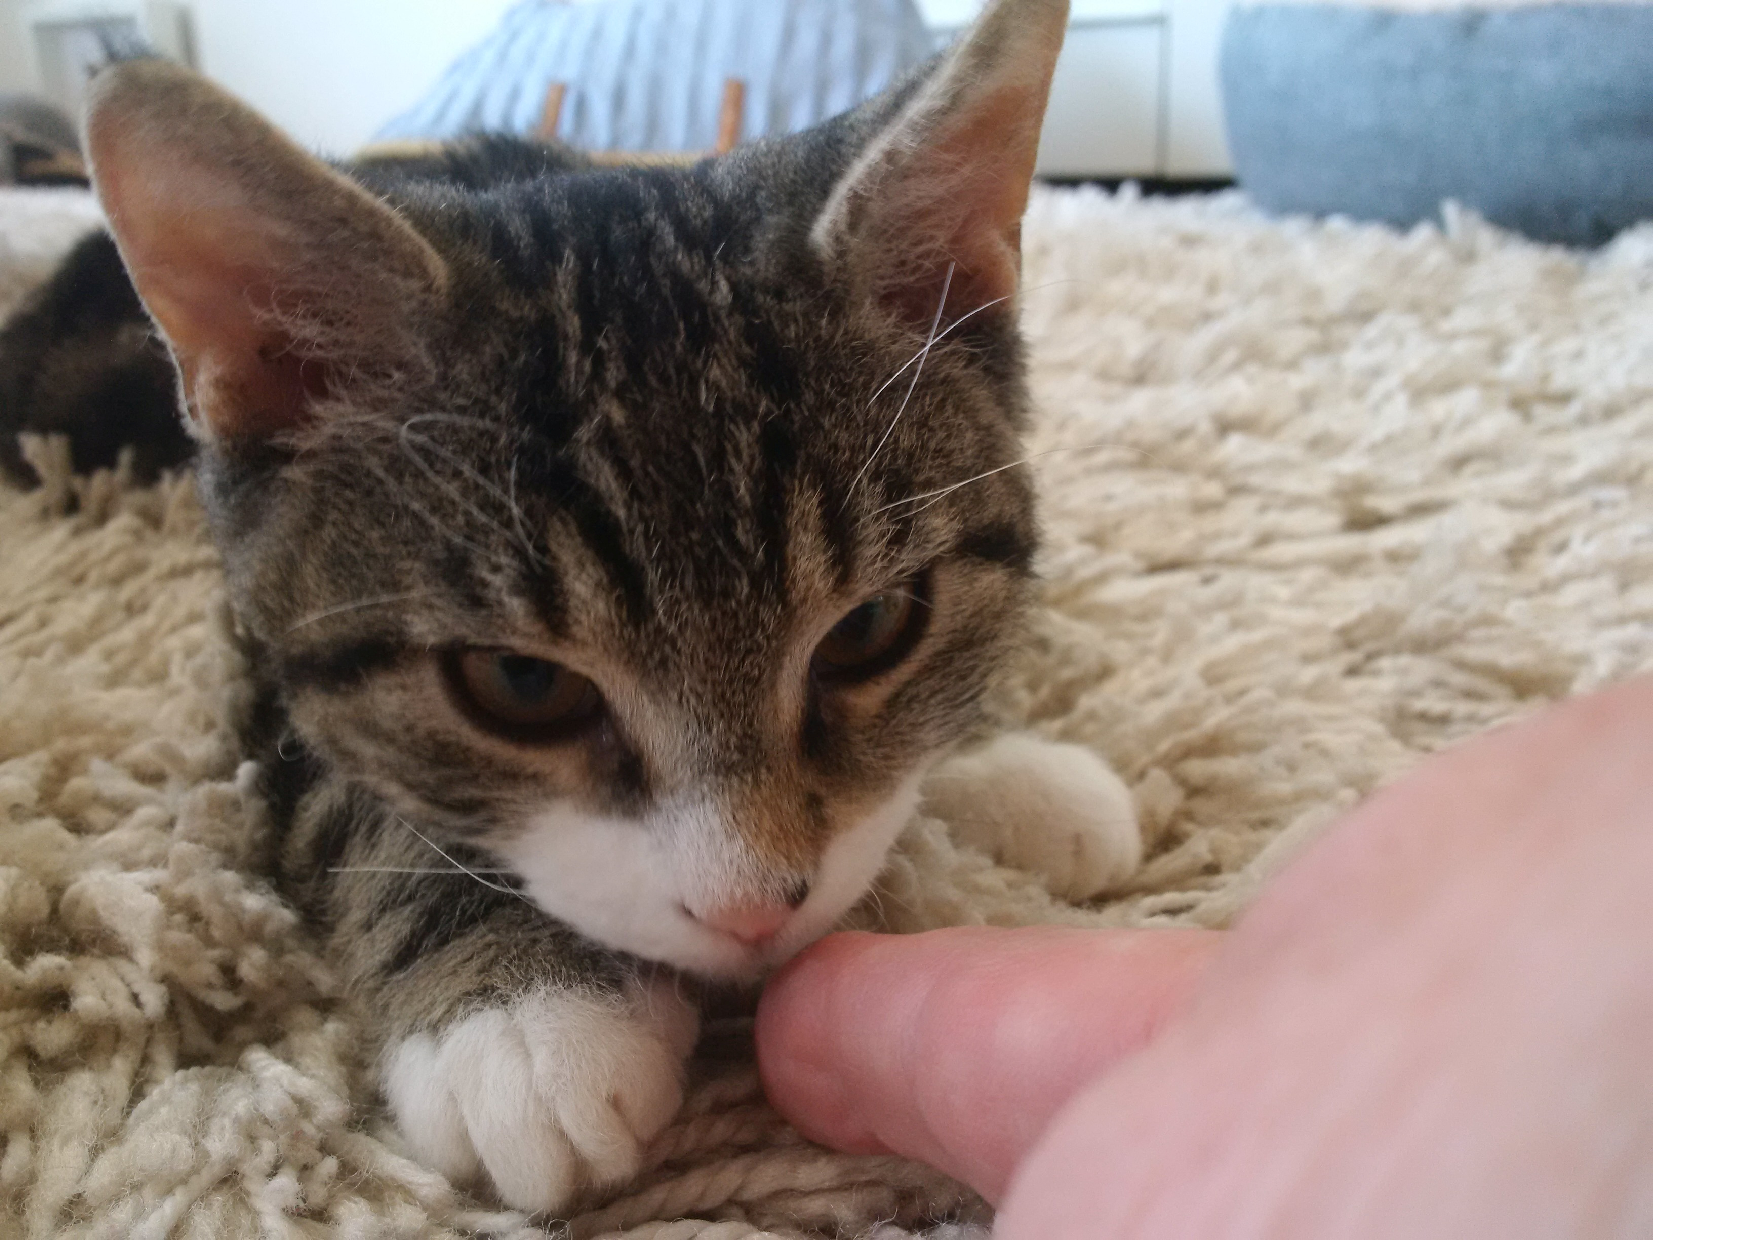
\includegraphics[width=200mm]{Bilder/UllisKater.pdf}}
	\put(4.5,-1){\parbox{720pt}{{\bf \small Abb. 1:} \small Beispielbild 1}}
	\end{picture}
\end{center}

		\end{multicols}
	}
}

% neuer Kasten
\vspace*{0.01\textheight}
%\Ovalbox
\widefbox
{
	\parbox{\textwidth}{
		\begin{multicols}{3}
			\textbf{\Large Kapitel B}\\

\blindtext

\begin{center}
	\begin{picture}(\spaltenbreite,16)
	\put(-1.9,1){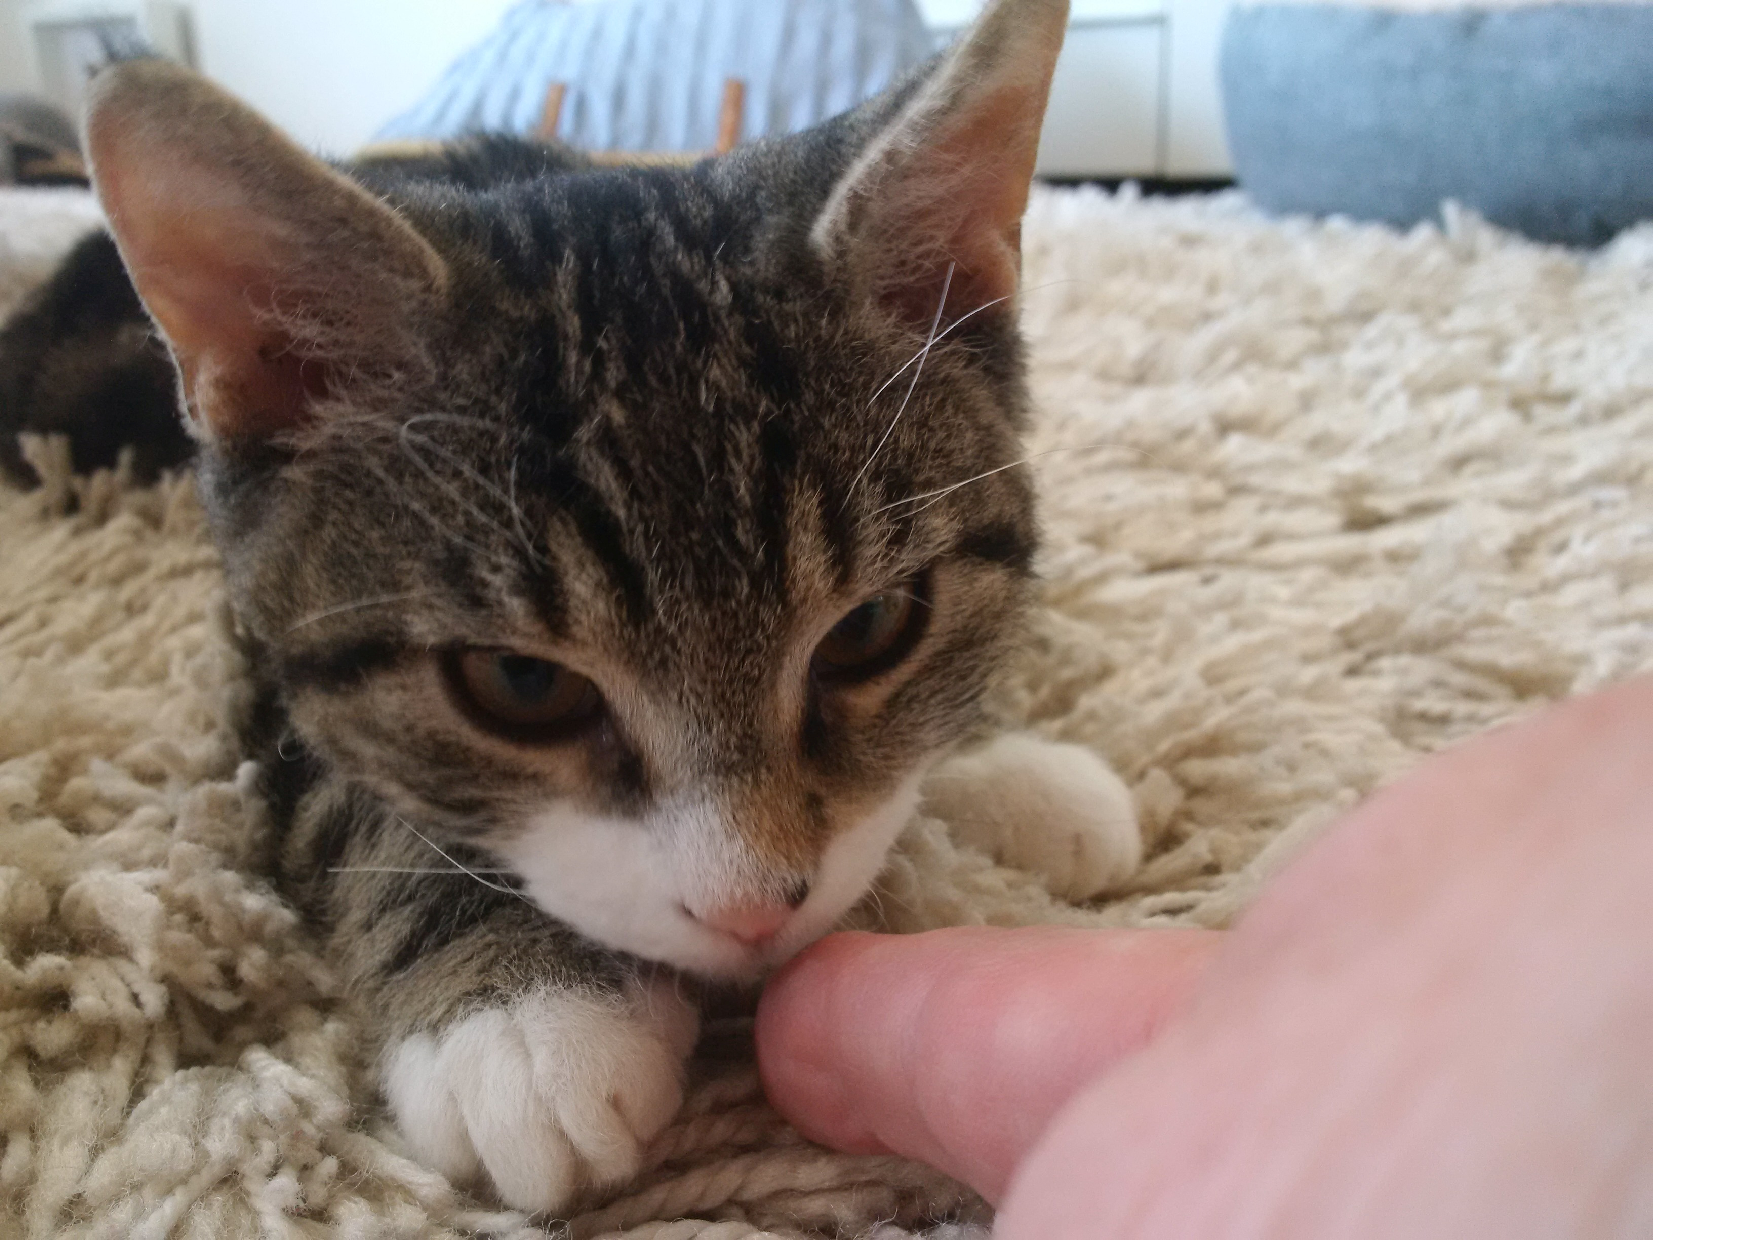
\includegraphics[width=200mm]{Bilder/UllisKater.pdf}}
	\put(4.5,-1){\parbox{720pt}{{\bf \small Abb. 2:} \small Beispielbild 2}}
	\end{picture}
\end{center}

		\end{multicols}
	}
}

\vspace*{0.01\textheight}
%\Ovalbox
\widefbox
{
	\parbox{\textwidth}{
		\begin{multicols}{3}
			\textbf{\Large Kapitel C}\\

\blindtext
		\end{multicols}
	}
}

\vspace*{0.01\textheight}
\widefbox
{
	\parbox{\textwidth}{
		\begin{multicols}{3}
			\textbf{\Large Kapitel D}\\

Erkenntnisse auflisten...\\

\blindlist{itemize}[3]
			\vfill
			\columnbreak				% erzeugt einen Spaltenumbruch falls mehrere Dateien eingebunden werden
			\nocite{*}
\printbibliography{}
		\end{multicols}
	}
}



\vspace*{15cm}										% gemäß der vorangehenden Textlänge einstellen, um die Fußzeile manuell zu verschieben
\begin{picture}(0,0)
\put(0,-1.4){\line(78,0){79.4}}
\put(0,-2.4){\textsf{\textbf{$\blacksquare${} Bachelorand: Max Mustermann, Betreuer: Prof. Dr. Dipl.-Ing. Ullrich Wenkebach, Studiengang: Biomedizintechnik, 2018}}}
\end{picture}
\end{document}